\documentclass{scrartcl}

\usepackage{graphicx}
\usepackage{amsmath}
\usepackage{wrapfig}
\usepackage{color}
\usepackage{sidecap}
\usepackage[format=plain,indention=1em,margin=0.05\textwidth]{caption}

\newcommand{\unit}[1]{\ensuremath{\operatorname{#1}}}
\newcommand{\um}{\unit{\mu m}}

\author{Peter Maunz}
\title{MQCO: Iontrapping experimental control software}

\begin{document}
\maketitle

\section{Overview}

\begin{figure}[htbp]
\begin{center}
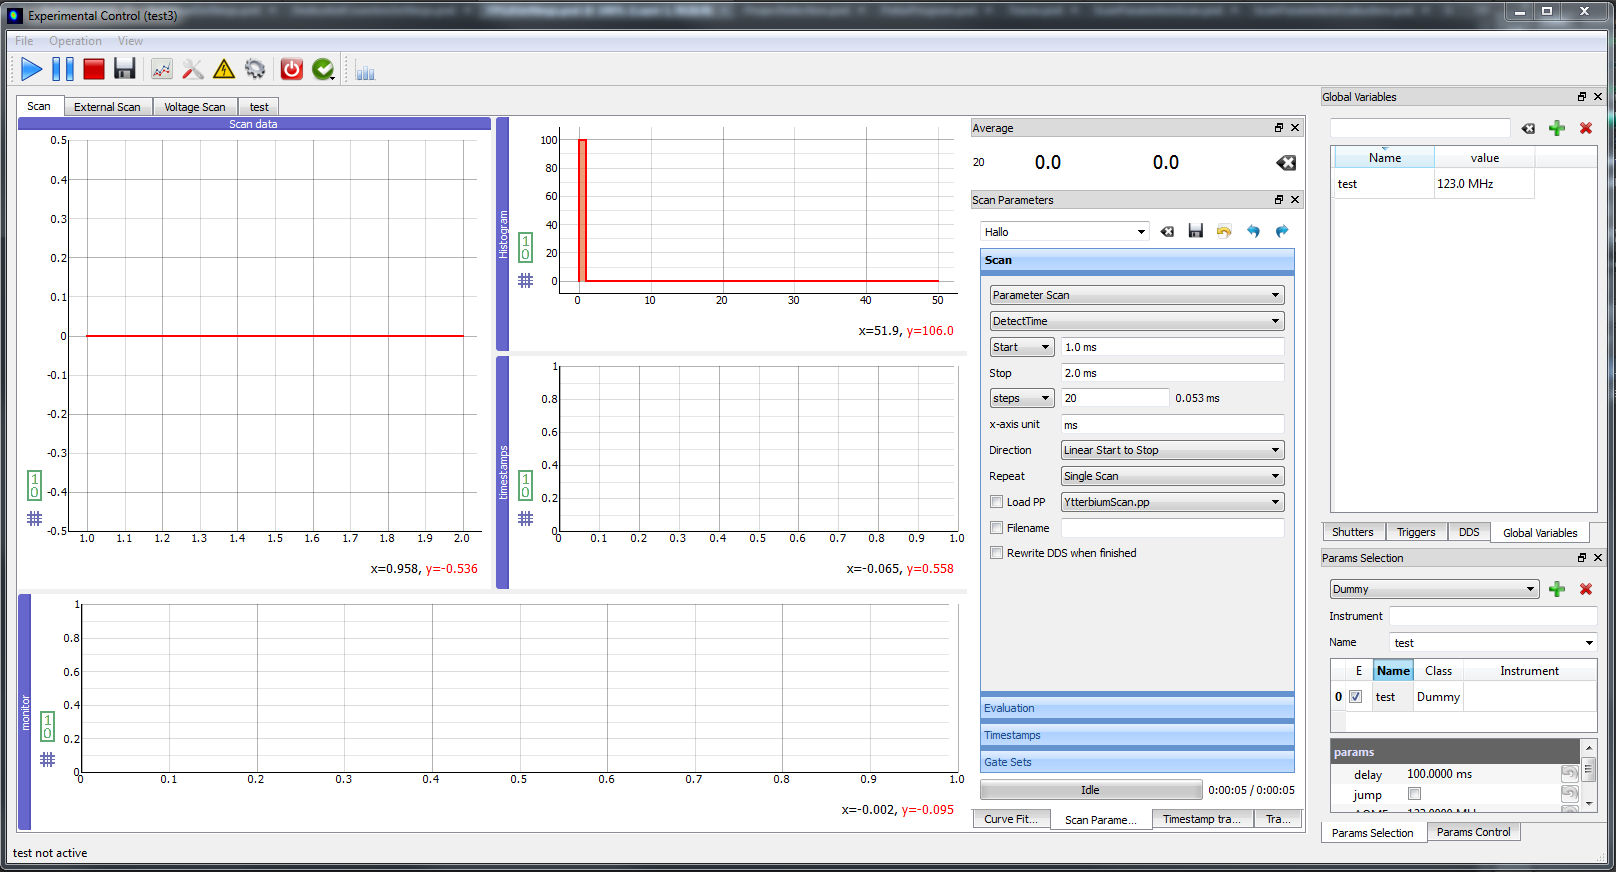
\includegraphics[width=\textwidth]{MainWindow}
\end{center}
\caption{\label{MainWindow} Main window.}
\end{figure}

\section{Project Selection}

\begin{SCfigure}
\centering
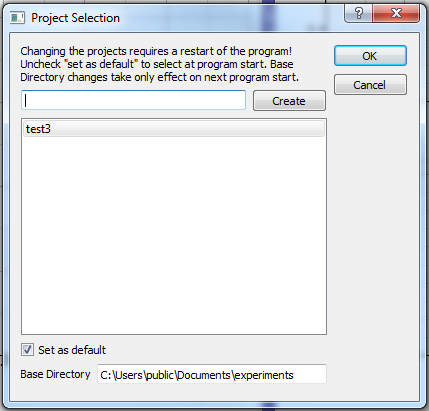
\includegraphics[width=0.48\textwidth]{ProjectSelection}
\caption{\label{ProjectSelection} Project Selection. Folders in the base directory afre considered projects. All configuration data and result data is saved in the project folder.}
\end{SCfigure}
The control program defines a "Base directory". The folders in the Base directory are considered Projects. Each Project has dedicated gui settings and data directories. The configuration data of the control program is saved in the folder .gui-config in the Project directory. It is recommended to create a folder "config" for the pulse program files and other configuration files. Data is saved by default in a directory structure consiting of year, month and day directories. This window is shown on first startup of the control program.

If "Set as default" is checked the control program will start with the default project. In this case the project can be changed by selecting File $\rightarrow$ Project.

\section{FPGA settings}
\begin{figure}[htbp]
\begin{center}
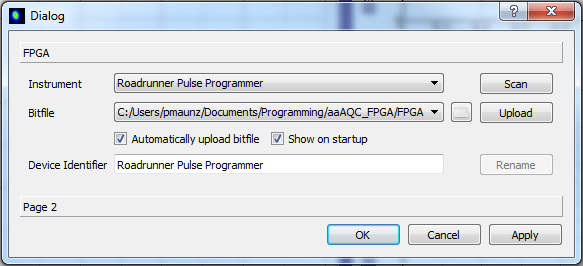
\includegraphics[width=0.7\textwidth]{FPGASettings}
\end{center}
\caption{\label{FPGASettings} Main window.}
\end{figure}

\section{Plot display}
\begin{figure}[htbp]
\begin{center}
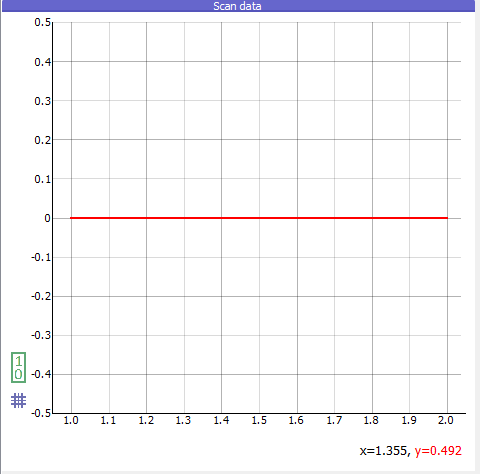
\includegraphics[width=0.8\textwidth]{ScanData}
\end{center}
\caption{\label{ScanData} Main window.}
\end{figure}


\section{Dedicated Counters}
\begin{figure}[htbp]
\begin{center}
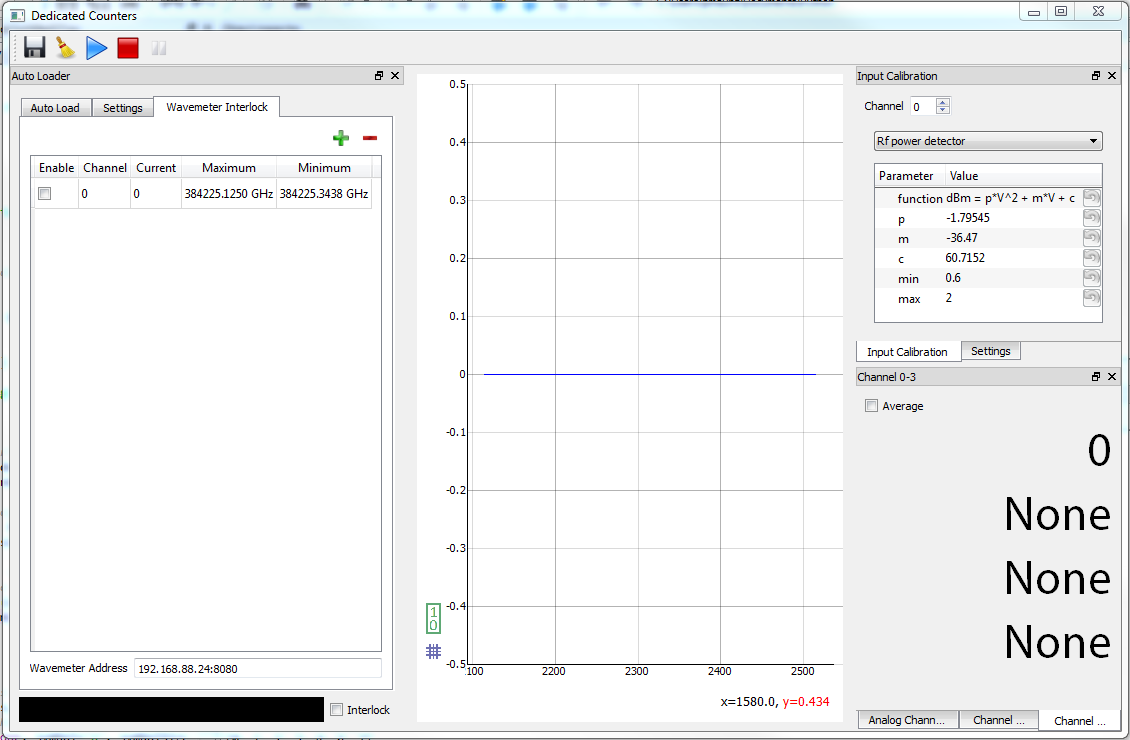
\includegraphics[width=\textwidth]{DedicatedCounters}
\end{center}
\caption{\label{DedicatedCounters} Main window.}
\end{figure}

\begin{figure}[htbp]
\begin{center}
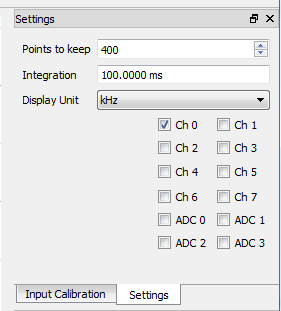
\includegraphics[width=0.5\textwidth]{DedicatedCountersSettings}
\end{center}
\caption{\label{DedicatedCountersSettings} Main window.}
\end{figure}



\subsection{Autoload}
\begin{figure}[htbp]
\begin{center}
\includegraphics[width=0.5\textwidth]{Autoload}
\end{center}
\caption{\label{Autoload} Main window.}
\end{figure}

\subsubsection{Settings}
\begin{figure}[htbp]
\begin{center}
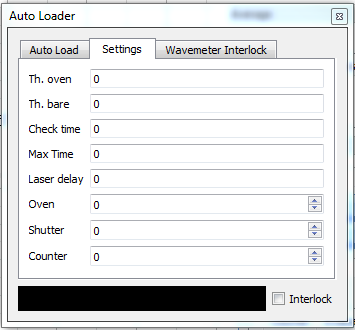
\includegraphics[width=0.5\textwidth]{AutoloadSettings}
\end{center}
\caption{\label{AutoloadSettings} Main window.}
\end{figure}



\subsubsection{Interlock}
\begin{figure}[htbp]
\begin{center}
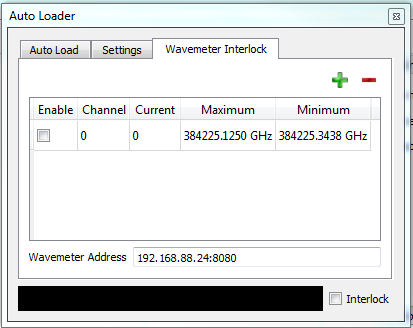
\includegraphics[width=0.7\textwidth]{WavemeterInterlock}
\end{center}
\caption{\label{WavemeterInterlock} Main window.}
\end{figure}

\subsection{Analog Inputs}
\begin{figure}[htbp]
\begin{center}
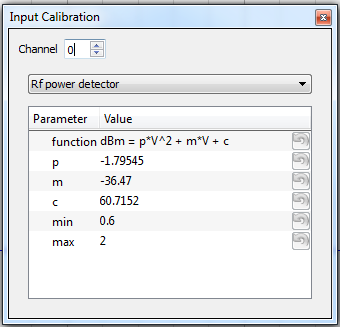
\includegraphics[width=0.5\textwidth]{AnalogInputCalibration}
\end{center}
\caption{\label{WavemeterInterlock} Main window.}
\end{figure}

\section{Global Variables}
\begin{figure}[htbp]
\begin{center}
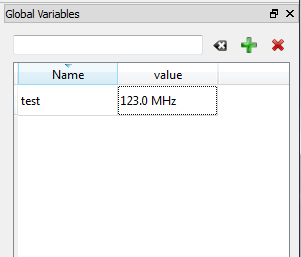
\includegraphics[width=0.5\textwidth]{GlobalVariables}
\end{center}
\caption{\label{GlobalVariables} Main window.}
\end{figure}


\section{Static settings}
\subsection{DDS}
\begin{figure}[htbp]
\begin{center}
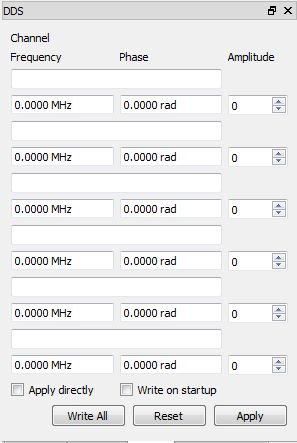
\includegraphics[width=0.5\textwidth]{DDS}
\end{center}
\caption{\label{DDS} Main window.}
\end{figure}

\subsection{Shutters}
\begin{figure}[htbp]
\begin{center}
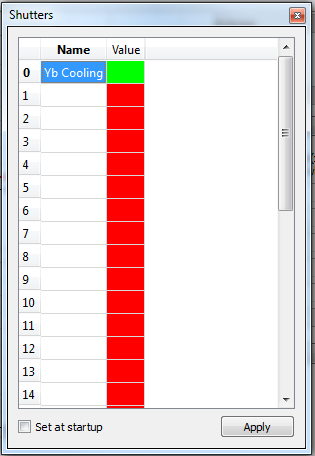
\includegraphics[width=0.4\textwidth]{Shutters}
\end{center}
\caption{\label{Shutters} Main window.}
\end{figure}

\subsection{Triggers}

\section{External Instruments}
\subsection{External Instrument Selection}
\begin{figure}[htbp]
\begin{center}
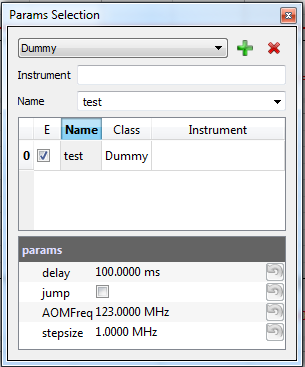
\includegraphics[width=0.5\textwidth]{ParamsSelection}
\end{center}
\caption{\label{ParamsSelection} Main window.}
\end{figure}

\subsection{External Instrument Control}
\begin{figure}[htbp]
\begin{center}
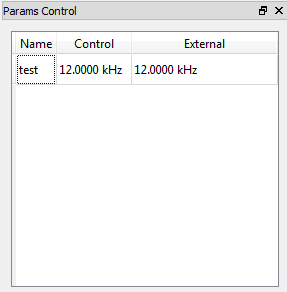
\includegraphics[width=0.5\textwidth]{ParamsControl}
\end{center}
\caption{\label{GlobalVariables} Main window.}
\end{figure}

\section{Pulse Program}
\begin{figure}[htbp]
\begin{center}
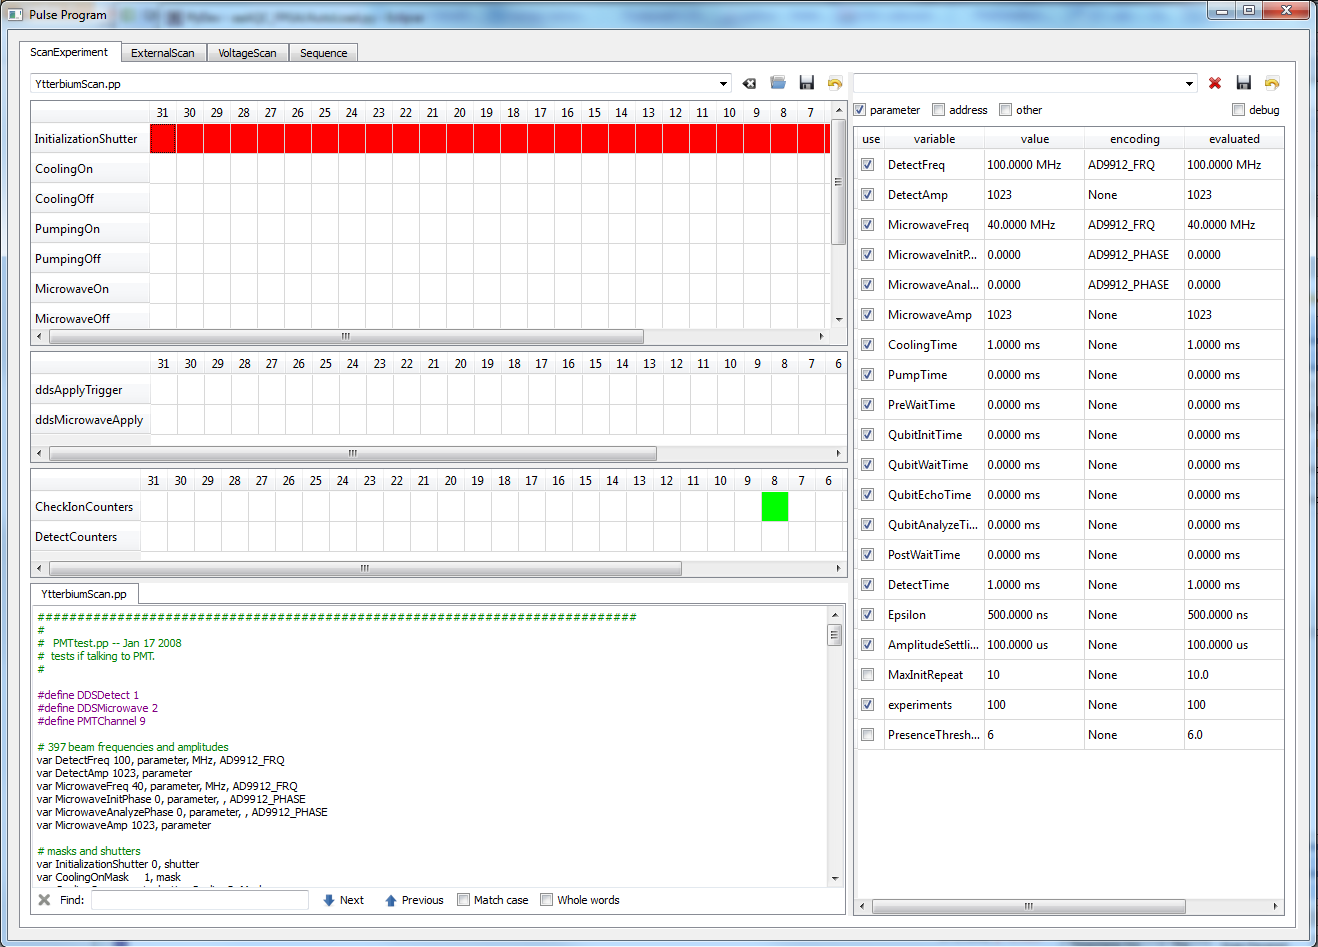
\includegraphics[width=\textwidth]{PulseProgram}
\end{center}
\caption{\label{PulseProgram} Main window.}
\end{figure}

\section{Scan configuration}
\subsection{Scan settings}
\begin{figure}[htbp]
\begin{center}
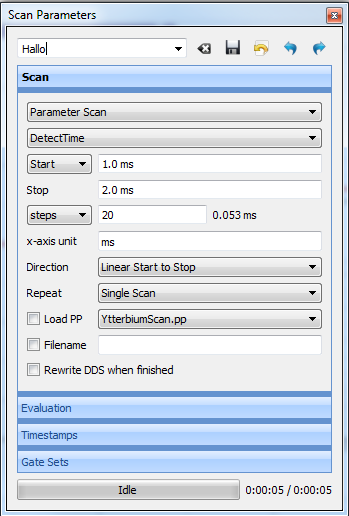
\includegraphics[width=0.5\textwidth]{ScanParametersScan}
\end{center}
\caption{\label{PulseProgram} Main window.}
\end{figure}

\subsection{Evaluation settings}
\begin{figure}[htbp]
\begin{center}
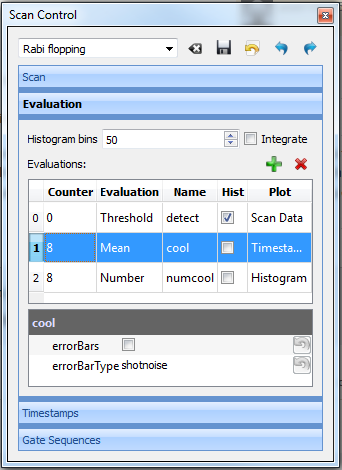
\includegraphics[width=0.5\textwidth]{ScanParametersEvaluation}
\end{center}
\caption{\label{PulseProgram} Main window.}
\end{figure}

\subsection{Timestamp settings}
\begin{figure}[htbp]
\begin{center}
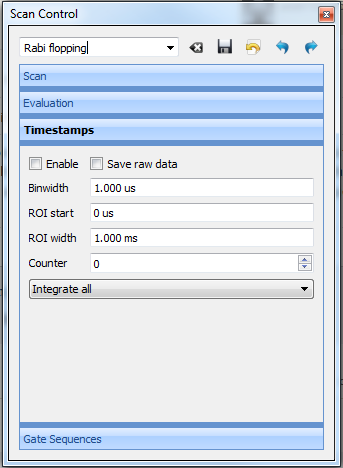
\includegraphics[width=0.5\textwidth]{ScanParametersTimestamps}
\end{center}
\caption{\label{PulseProgram} Main window.}
\end{figure}


\subsection{Gate Sets settings}
\begin{figure}[htbp]
\begin{center}
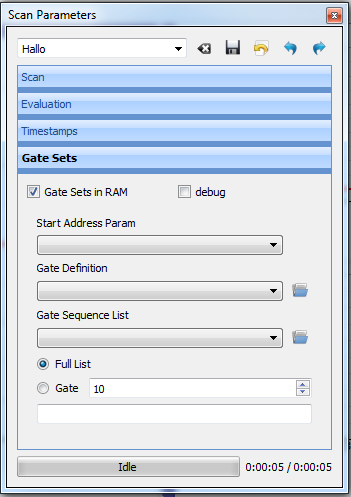
\includegraphics[width=0.5\textwidth]{ScanParametersGateSets}
\end{center}
\caption{\label{PulseProgram} Main window.}
\end{figure}

\section{Curve fitting}
\begin{figure}[htbp]
\begin{center}
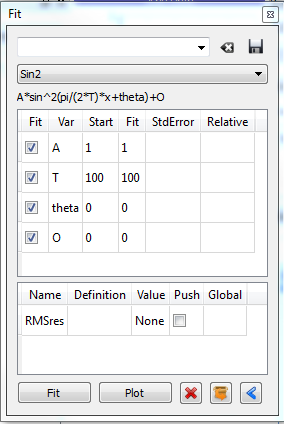
\includegraphics[width=0.5\textwidth]{CurveFitting}
\end{center}
\caption{\label{AutoloadSettings} Main window.}
\end{figure}

\section{Traces}
\begin{figure}[htbp]
\begin{center}
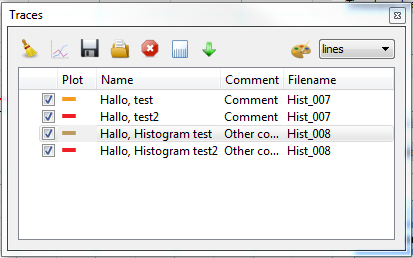
\includegraphics[width=0.5\textwidth]{Traces}
\end{center}
\caption{\label{AutoloadSettings} Main window.}
\end{figure}


\end{document}